\pr At the Savior’s command and formed by divine teaching, we dare to say:

\begin{center}
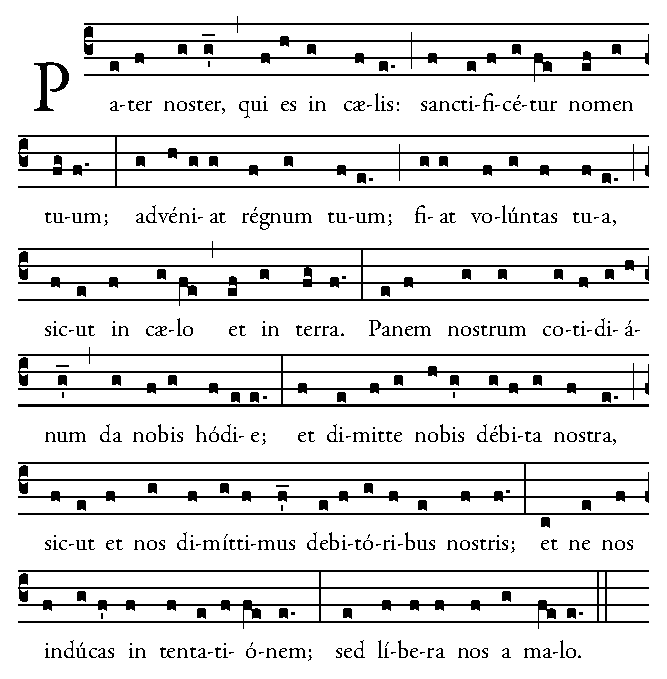
\includegraphics[width=.9\textwidth]{src/ordinario/pater.eps}
\end{center}

\be Our Father, who art in heaven,\redast hallowed be thy name;\redast thy kingdom come,\redast thy will be done on earth as it is in heaven.\redast Give us this day our daily bread,\redast and forgive us our trespasses,\redast as we forgive those who trespass against us;\redast and lead us not into temptation,\redast but deliver us from evil.

\pr Deliver us, Lord, we pray, from every evil, graciously grant peace in our days, that, by the help of your mercy, we may be always free from sin and safe from all distress, as we await the blessed hope and the coming of our Savior, Jesus Christ.

\be For the kingdom, the power and the glory are yours now and for ever.

\pr Lord Jesus Christ, who said to your Apostles: Peace I leave you, my peace I give you; look not on our sins, but on the faith of your Church, and graciously grant her peace and unity in accordance with your will. Who live and reign for ever and ever.

\be Amen.

\pr The peace of the Lord be with you always.

\be And with your spirit.

\pr Let us offer each other the sign of peace.

\be Lamb of God, you take away the sins of the world,\redast have mercy on us.\\
\indent\be Lamb of God, you take away the sins of the world,\redast have mercy on us.\\
\indent\be Lamb of God, you take away the sins of the world,\redast grant us peace.

\pr Behold the Lamb of God, behold him who takes away the sins of the world. Blessed are those called to the supper of the Lamb.

\be Lord, I am not worthy that you should enter under my roof, but only say the word and my soul shall be healed.

\pr Let us pray.

\pr Keep safe, O Lord, we pray, those whom you have saved by your kindness that, redeemed by the Passion of your Son, they may rejoice in his Resurrection. Who live and reigns for ever and ever.

\be Amen.